
%
%  void-input - easy report template for included file
%  EDIT THE LINE ABOVE FOR DOCUMENTATION OF THIS FILE, then delete this line! 
%         

%

% ============================================================
% --- texstudio magic comment: 
% !TEX encoding = UTF-8
% !TeX program = pdflatex
%% !TeX program = xelatex
% !TeX root = "cognome-tesina.tex"
% %  !TeX spellcheck = en_US
% !TeX spellcheck = it_IT


% ====================================================================


\chapter{Task 1}
This first task was not complicated in the selection of the type of cluster to be used or in its implementation but it was very long in the selection of the image preprocessing methods and in the selection of the correct values. In the end I chose to use a mix of both before and after segmentation to remove the noise that plagued the second and third images. I used Gaussian blur, Erosion and Dilation also increasing the brightness of the image to remove the darkest areas. As the main method instead I used Otsu’s thresholding. After numerous unsuccessful attempts to try the different values I implemented sliders as in the first task of lab 4 to find the correct parameters and then insert them in the code. The Figure \ref{fig:1a} is the one that gave the best result while the other 2 (Figure \ref{fig:1c} and Figure \ref{fig:1e} still kept some noise).

\begin{figure}[h]
	\centering
	\begin{minipage}{0.45\textwidth}
		\centering
		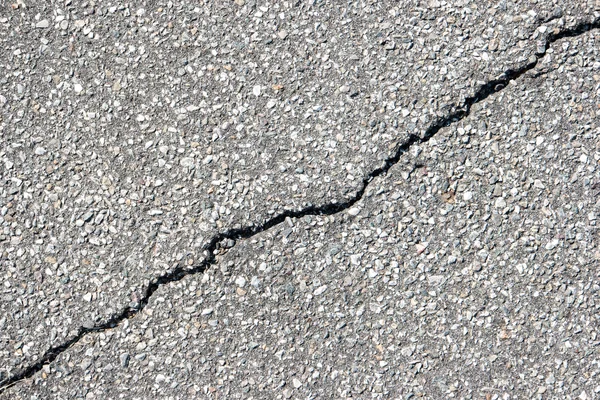
\includegraphics[width=\linewidth]{images/source/original/1}
		\caption{First image before segmentation.}
		\label{fig:1a}
        \end{minipage}
        \hspace{0.05\textwidth}
        \begin{minipage}{0.45\textwidth}
        		\centering
		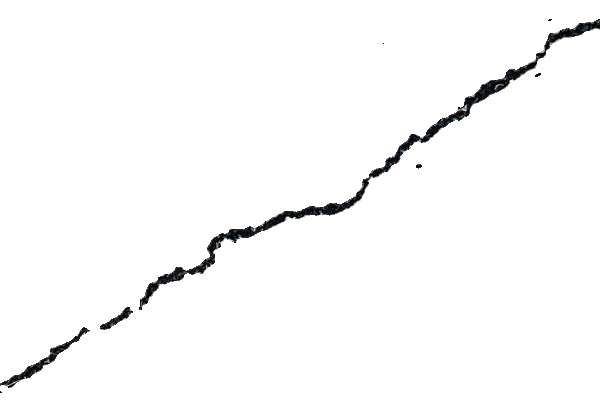
\includegraphics[width=\linewidth]{images/source/task1/1}
		\caption{First image after segmentation.}
		\label{fig:1b}
        \end{minipage}
\end{figure}

\begin{figure}[h]
	\centering
	\begin{minipage}{0.45\textwidth}
		\centering
		
\includegraphics[width=\linewidth]{images/source/original/2}
		\caption{Second image before segmentation.}
		\label{fig:1c}
        \end{minipage}
        \hspace{0.05\textwidth}
        \begin{minipage}{0.45\textwidth}
        		\centering
		
\includegraphics[width=\linewidth]{images/source/task1/2}
		\caption{Second image after segmentation.}
		\label{fig:1d}
        \end{minipage}
\end{figure}

\begin{figure}[h]
	\centering
	\begin{minipage}{0.45\textwidth}
		\centering
		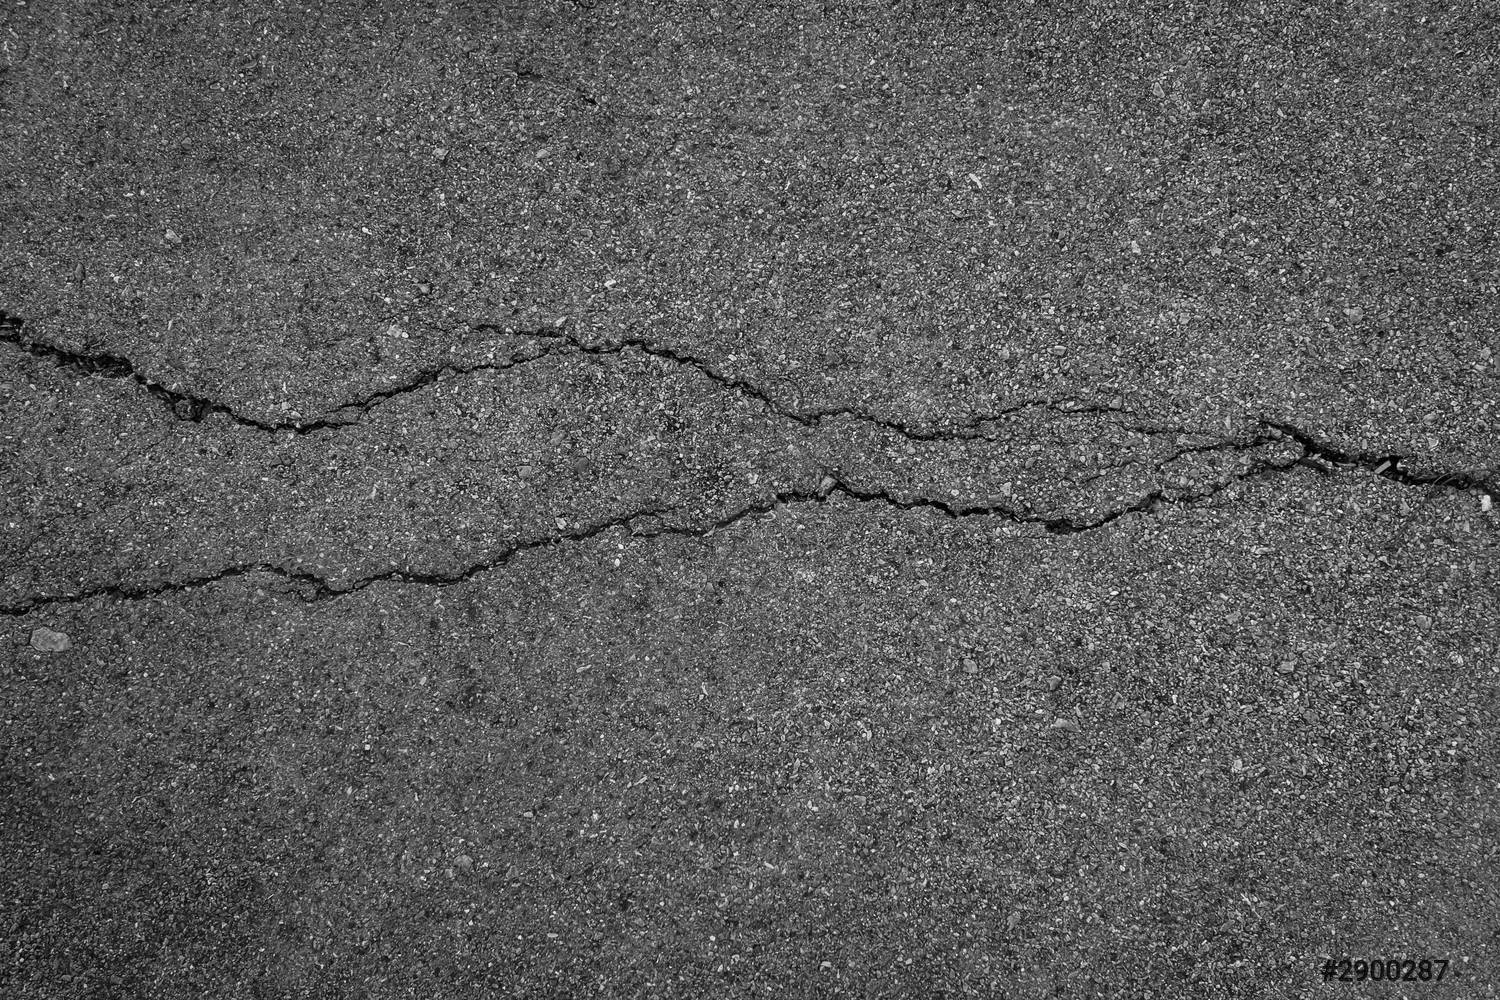
\includegraphics[width=\linewidth]{images/source/original/3}
		\caption{Third image before segmentation.}
		\label{fig:1e}
        \end{minipage}
        \hspace{0.05\textwidth}
        \begin{minipage}{0.45\textwidth}
        		\centering
		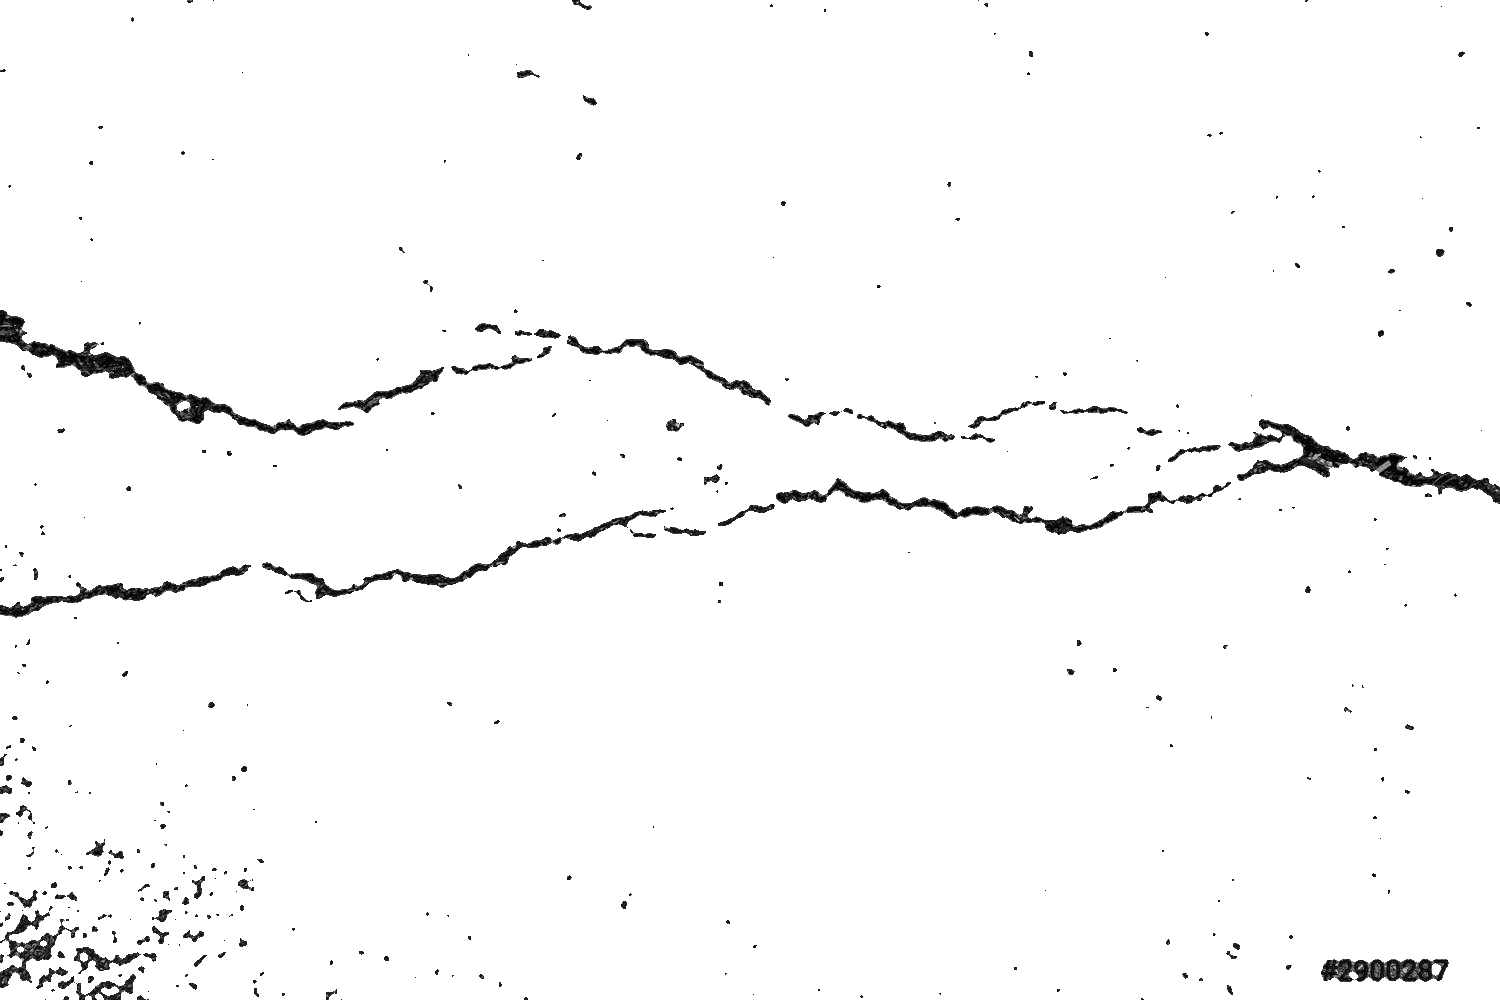
\includegraphics[width=\linewidth]{images/source/task1/3}
		\caption{Third image after segmentation.}
		\label{fig:1f}
        \end{minipage}
\end{figure}

\chapter{Task 2}
I spent the majority of the time to improve the kmeans performance as much as possible so as to effectively classify the image. Finally I also used cv::erode to ”delete” useless elements in the image. Unfortunately I couldn’t overdo it otherwise I would have missed too many items. In this case a small portion of a box was misclassified and I couldn’t fix it without increasing the erosion too much. (However, a possible solution could be to use cv::Houghlines to delimit the line of the roads so as to fix the missclassified elements before this line with a for loop.) As can be seen in Figure \ref{fig:2b}, the image without erosion it has many badly classified elements. While in Figure \ref{fig:2c} it is possible to see the elements classified correctly with the exception of the box previously described.

\begin{figure}[h]
	\centering
	\begin{minipage}{0.45\textwidth}
		\centering
		
\includegraphics[width=\linewidth]{images/source/original/4}
		\caption{Original image.}
		\label{fig:2a}
        \end{minipage}
        \hspace{0.05\textwidth}
        \begin{minipage}{0.45\textwidth}
        		\centering
		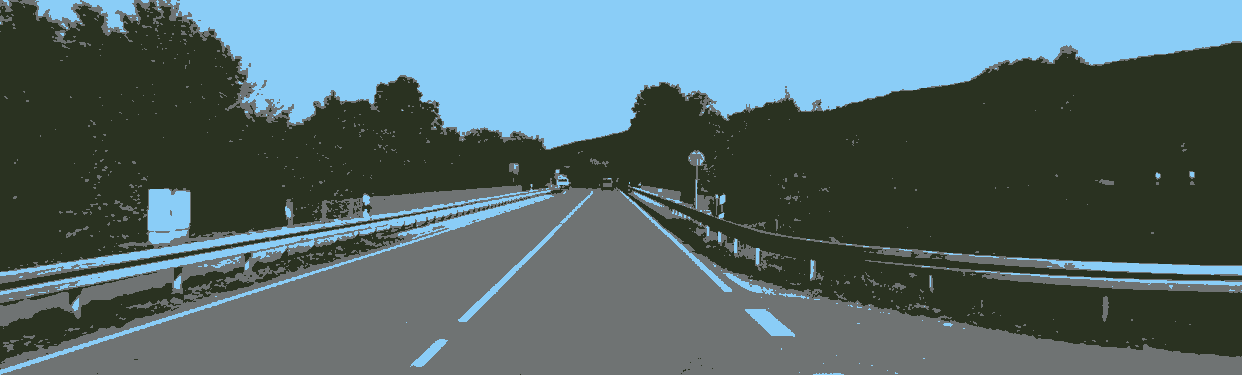
\includegraphics[width=\linewidth]{images/source/task2/1}
		\caption{Image without cv::erode.}
		\label{fig:2b}
        \end{minipage}
\end{figure}

\begin{figure}[h]
	\centering
        \begin{minipage}{0.9\textwidth}
        		\centering
		
\includegraphics[width=\linewidth]{images/source/task2/2}
		\caption{Final image with cv::erode.}
		\label{fig:2c}
        \end{minipage}
\end{figure}

\chapter{Task 3}
I tried Otsu’s thresholding and k-means in different variations but unfortunately none of them worked. The shirts were always clustered incorrectly. In the end I opted for a simple method, that is through the color range. I have selected the color range of the shirts. Then I looked for the circles in the image so as to find the ball which, having a similar color to the shirts, ended up in the main mask. Found the ball with HoughCircles I built a mask around it to remove it from the elements of my interest. In the end I then used cv::bitwise and to remove everything that is not of interest to me from the image and return the final image with only the shirts. In the images below (Figure \ref{fig:3a} and Figure \ref{fig:3b}) you can see the starting image and the final result.
Note: I tried to use cv::bitwise but when I compiled with cmake the image came out differently so I used a double for loop.

\begin{figure}[h]
	\centering
	\begin{minipage}{0.45\textwidth}
		\centering
		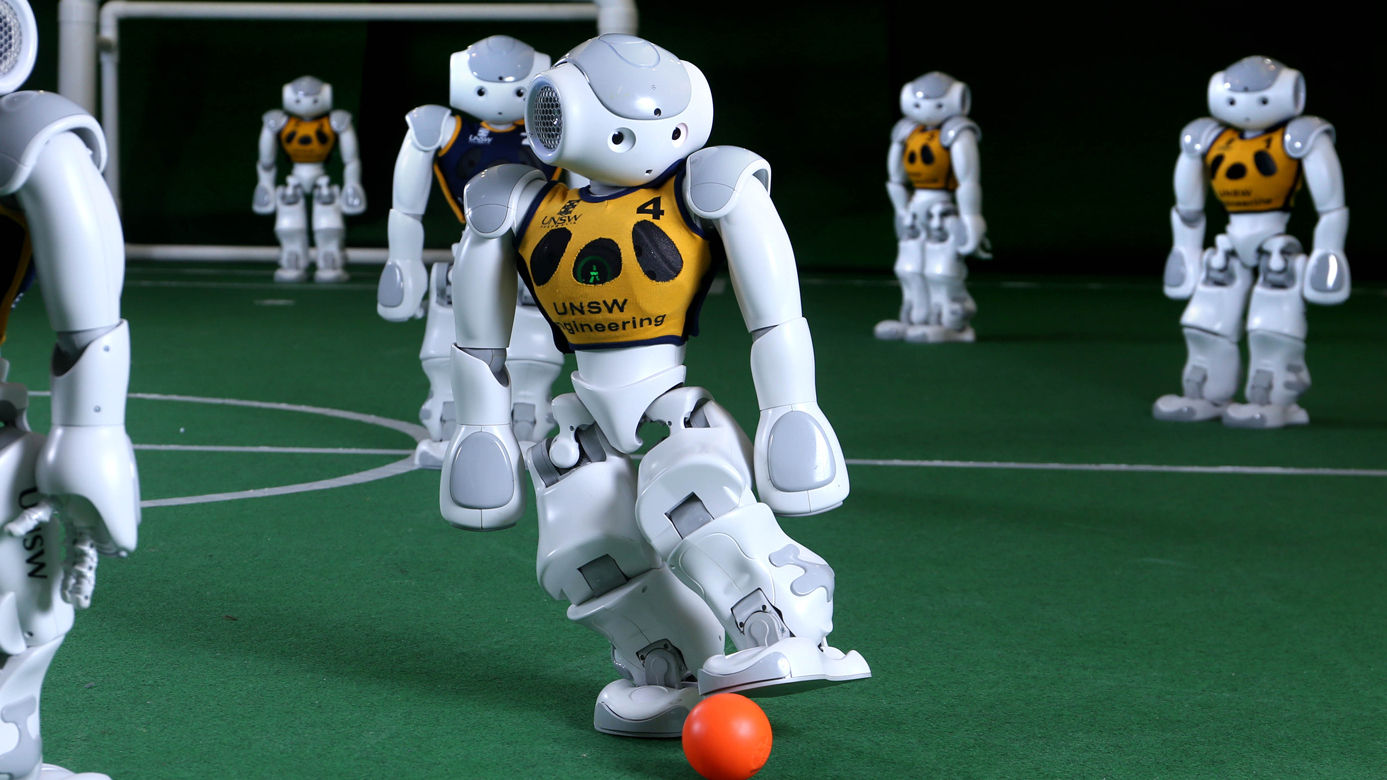
\includegraphics[width=\linewidth]{images/source/original/5}
		\caption{Original image.}
		\label{fig:3a}
        \end{minipage}
        \hspace{0.05\textwidth}
        \begin{minipage}{0.45\textwidth}
        		\centering
		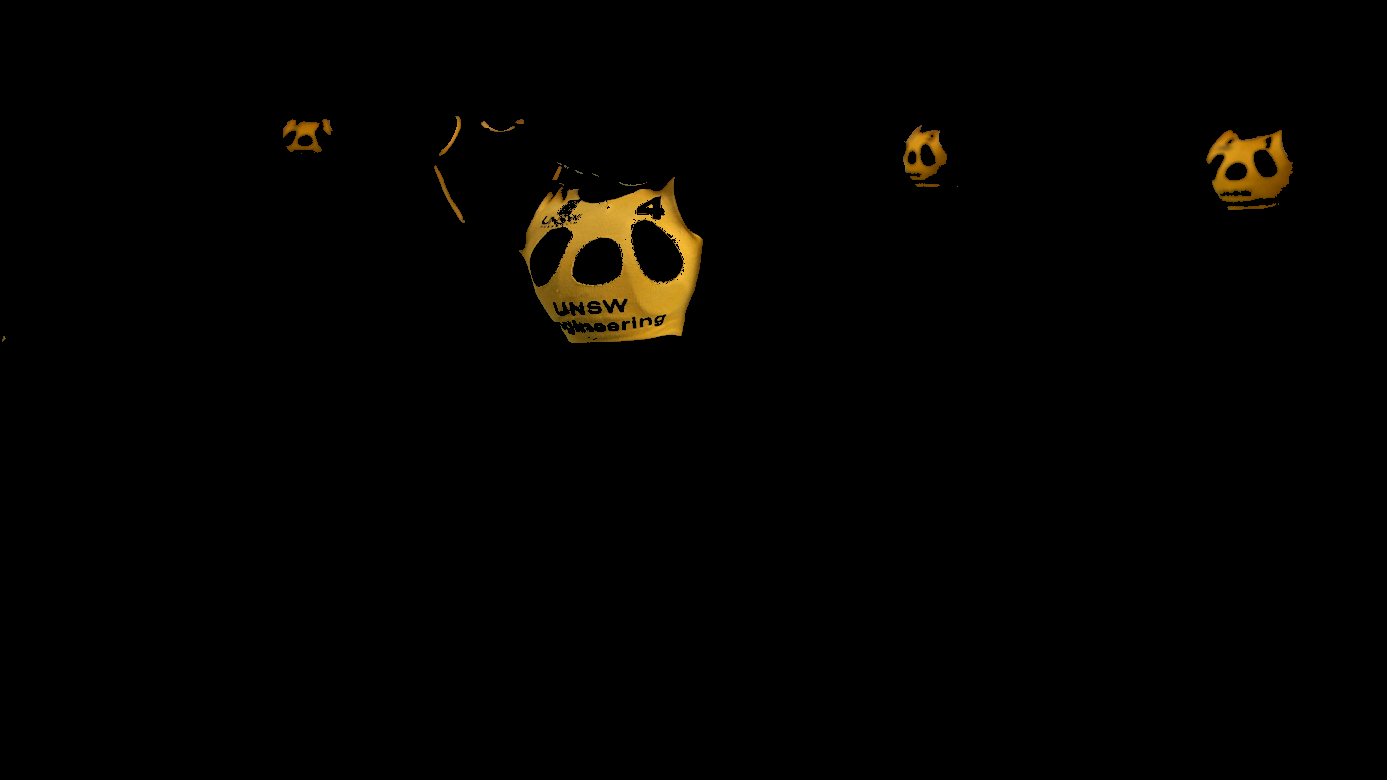
\includegraphics[width=\linewidth]{images/source/task3/1}
		\caption{Final Image.}
		\label{fig:3b}
        \end{minipage}
\end{figure}




% ====================================================================

% ====================================================================
% memo available commands
% ====================================================================
% easyrep: summary of provided macros
%
% \Title{text}     defines the document title 
% \Subtitle{text}  defines the subtitle
% \Author{text}    defines the author string
% \Date{text}      defines a date string
% \printCover      print a cover page using above information
%
% --- text styles
% \tDef{text}      definition (generic) 
% \tDefObj{text}   definition (the ter being defined)
% \tDefTxt{text}   definition (the statement defining the term) 
% \tRemark{text}   remarked text
% \tREMARK{text}   highly remarked text 
% \tLoud{text}     shouted text! 
% \tCode{text}     inline code text
% \tLatin{text}    latin text
% \tForeign{text}  foreign language text 
% \tExample{text}  example 
% \tStandard{text} a recommendation 
% \tQuote{text}    a quoted text 
% \tQuoteFig{text} a quoted text referring to a figure 
% \tConcept{text}  an important concept  
% \tBeginPar{text} highlighted text 
%                  at the beginning of a paragraph 
%
% ---environments
% \begin{quoteStandard} text... \end{quoteStandard}
%    print text to be quoted, e.g. sentences from 
%    a recommendation
%
% \begin{quoteRemark} text... \end{quoteRemark}
%    similar to quoteStandrd, but the text is more marked
%
%  
% --- typo accelerators
% \qmo             opening quotation mark (use \qmo{})
% \qmc             closing quotation mark (use \qmc{})
% \th  emphasises "th"
% \ie  slanted "i.e."
% \eg  slanted "e.g."
% \es  slanteg "ad es."
% \octave   "octave" in \tCode style
% \matlab   "matlab"
% \labview  "labVIEW"
% \latex    "LaTeX" (just the text!)
%
% --- math typo accelerators
% \v{math text}  underlines the math text (useful for vector) 
%
% --- debug commands
% \debugTextStyles        print a table showing text styles
% \debugPrintCharacters   print a table of characters
% \Vispa                  print some text (to fill)  
% \Vispas                 more filling text
% ====================================================================
